\section{Coulomb-Nuclear Interference}
\label{sec:coulomb}

%----------------------------------------------------------------------------------------------------

\subsection{Theoretical Framework}
\label{sec:cni_framework}

In this section the different components of the combined elastic scattering amplitude, already briefly outlined in the introduction, are discussed in more detail. In particular, the possible choices for theoretically unknown terms are explained.

%------------------------------------------------------------------
\subsubsection{Coulomb Amplitude}
%
The Coulomb amplitude can be calculated from QED (e.g.~Section 3.2 in \cite{block06}), using empirical electric and magnetic form factors of the proton (e.g.~\cite{puckett10}). It can be shown (e.g.~Section 1.3.1 in~\cite{jan_thesis}) that, at low $|t|$, the effect of both form factors can be described by a single function ${\cal F}$. 


\subsubsection{Nuclear Amplitude}
%
Since the nuclear amplitude can presently not be calculated from first principles, its phenomenological description will be discussed.

The {\bf modulus} is closely related to the differential cross-section and thus strongly constrained by experimental observations outside the Coulomb and CNI region. Following especially~\cite{8tev-90m}, the modulus for $|t|~\lesssim~0.2$, i.e. well below the diffractive minimum, will be parametrised as:
\begin{equation}
\label{eq:nuc mod}
| {\cal A}^{\rm N}(t) | = a \exp\left( \sum\limits_{n}^{N_b} b_n t^n \right)\ ,
\end{equation}
%\todo{for $|t| < 0.2$, what about higher $|t|$'s?}\\
where $N_b$ gives the number of free parameters in the exponent. This implicitly extends the exponential behaviour to the regions where the (pure nuclear) cross-section cannot be observed. Although there is no rigorous justification, and therefore it stands as an assumption, it is compatible with many theoretical models.

For the {\bf phase} of the nuclear amplitude, there is little experimental guidance and therefore several theory-motivated choices will be assumed and tested.

\begin{itemize}
% ***
\item A {\it constant phase} is obviously the simplest choice:
%
\begin{equation}
\label{eq:nuc phase const}
\arg {\cal A}^{\rm N}(t) = \hbox{const.}
\end{equation}
Note that this is equivalent to a strict proportionality of real and imaginary part of the amplitude at all $t$.
%
% ***
\item The {\it standard phase} parametrisation,
\begin{equation}
\label{eqn:nuc_phase_standard}
\arg {\cal A}^{\rm N}(t) = p_{0} + \arctan \left(\frac{|t|-|t_{0}|}{\tau}\right) -  \arctan \left(\frac{-|t_{0}|}{\tau}\right) \: ,
\end{equation}
implements the main features of many theoretical models -- almost imaginary amplitude in the forward direction ($p_0 \approx \pi/2$) while almost purely real in the (first) diffraction dip 
($\arg {\cal A}^{\rm N}(t) \approx \pi$ at $t = t_{0}$). \todo{[to be corrected]}

% ***
%
\item The parametrisation by {\em Bailly et al.}~\cite{bailly87} \todo{[to be written]}
\begin{equation}
\label{eq:nuc phase std}
	%\arg {\cal A}^{\rm N}(t) = {\pi\over 2} - \arctan {\rho_0\over 1 - {t\over t_{\rm d}}},\ \rho_0 = {1\over \tan p_0}
	\arg {\cal A}^{\rm N}(t) = \arctan \left[ \tan p_0 \left(1 - {t\over t_{\rm d}} \right) \right]\ ,
\end{equation}
where $p_0$ determines the phase value at $t=0$ and $t_{\rm d} \approx -0.53\un{GeV^2}$ gives the position of the diffractive minimum at $8\un{TeV}$ (preliminary result from $90\un{m}$ data).
%
% ***
\item The {\it peripheral phase} \cite{kl94} \todo{newer ref - if we ever get one} provides an alternative to the above descriptions. Its parametrisation

\todo{update values, range?}\\
\todo{if range used: several options with different level of peripherality as assumption - the RMS of b el was initially fixed by Vojtech - it is a cause not consequence}

\begin{equation}
\label{eq:nuc phase per}
\arg {\cal A}^{\rm N}(t) = p_0 - A \exp\left[ \kappa \left( \log {t\over t_{\rm m}} - {t\over t_{\rm m}} + 1 \right) \right]
\end{equation}
results in a peak at $t_{\rm m} \approx -0.310\un{GeV^2}$, with amplitude $A \approx 5.53$ and width controlled by $\kappa \approx 4.01$.
\end{itemize}
%
\begin{figure*}
\begin{center}
% TODO: file not in the repository
%\includegraphics[width=\textwidth]{phase_illustration.pdf}
\vskip-3mm
\caption{}
\label{fig:phase_illustration}
\end{center}
\end{figure*}

It should be noted that the phase has decisive influence on the amplitude behaviour in the space of impact parameter, $b$, see e.g.~Section 3 in~\cite{klk02}. It can be quantified by evaluating the root-mean-squares (RMS) of $b$ for elastic and inelastic collisions. The constant and standard phase lead to elastic collisions more central (smaller RMS) than the inelastic ones. The peripheral phase can yield a description with the opposite hierarchy, which is argued more natural by some authors (e.g. Section~4 in~\cite{kl96}).

%----------------------------------------------------------------------------------------------------
\subsubsection{Coulomb-Nuclear Interference Formulae}

The {\bf simplified West-Yennie formula (SWY)} \cite{wy68} is derived in the framework of perturbative QFT by evaluating the lowest-order Feynman diagrams that comprise both nuclear and Coulomb interactions. In this approach, the interference is reduced to an additional phase between the Coulomb and nuclear amplitudes. Moreover, several approximations were used in the derivation. First, in order to avoid integrating over off-mass-shell contributions to the nuclear amplitude (purely known), very slow variation of the nuclear amplitude phase was assumed: $\arg {\cal A}^{\rm N} \approx \hbox{const}$. Then, in order to obtain a closed-form expression, the exponential slope of the nuclear modulus
\begin{equation}
B^{\rm N}(t) = {\d \log |{\cal A}^{\rm N}|^2 \over \d t}
\end{equation}
was assumed constant. The original formula did not contain the electromagnetic form factor ${\cal F}$, it was added later by hand:
\begin{equation}
\label{eq:int swy}
	\begin{aligned}
		{\d\sigma\over \d t}^{\rm C+N} &= {\pi (\hbar c)^2 \over s p^2} \left | {\alpha s\over t} {\cal F}^2 \e^{\I\alpha \Phi(t)} + {\cal A}^{\rm N} \right |^2\ ,\cr
		\Phi(t) &= - \left( \log {B |t|\over 2} + \gamma \right)\ ,\cr
	\end{aligned}
\end{equation}
where $\gamma \doteq 0.577$ is the Euler constant. Despite the many limitations, the formula has extensively been used in past data analyses. For backward-comparison reasons we consider it also in this report.

The {\bf Kundr\' at-Lokaj\' i\v cek formula (KL)} \cite{kl94} was derived in an impact parameter formalism and it is based on the additivity of eikonals. The derivation poses no limitations on nuclear amplitude and the formula naturally incorporates the electromagnetic form-factor. In this treatment, the interference effect goes beyond a single phase, the $\Psi$ quantity is complex, in general:
\begin{equation}
\label{eq:int kl}
	\begin{aligned}
		{\d\sigma\over \d t}^{\rm C+N} &= {\pi (\hbar c)^2 \over s p^2} \left | {\alpha s\over t} {\cal F}^2 + {\cal A}^{\rm N} \e^{\I\alpha \Psi(t)} \right |^2\ ,\cr
		\Psi(t) &= 
			- \int \d t'\, \log {t'\over t} {\d\phantom{t'}\over \d t'} {\cal F}^2(t') \cr
		&\phantom{=} + \int \d t' \left( {{\cal A}^{\rm N}(t') \over {\cal A}^{\rm N}(t)} - 1 \right) { I(t, t')\over 2\pi }
			\ ,\cr
		I(t, t') &= \int_0^{2\pi} \d\phi\ {{\cal F}^2(t'')\over t''}\ , \cr
		t'' &= t + t' + 2\sqrt{t\, t'} \cos\phi\ ,\cr
	\end{aligned}
\end{equation}
where the $t$ integrations go over the entire kinematically allowed region.

Calculation engine \cite{elegent}, using form-factor of Puckett et al.~\cite{puckett10}

%----------------------------------------------------------------------------------------------------
%----------------------------------------------------------------------------------------------------
\subsection{Data analysis}
\label{sec:cni_anal}

\subsubsection{Jan's notes}

\> nuclear modulus
\>> anchored to $90\un{m}$ data at $|t| > 0.2\un{GeV^2}$ for stability of integrations in \ref{eq:int kl}
\>> considering 1, 2 and 3 parameters, then no improvement of $\chi^2$

\> with the presented data not possible to distinguish between different models/assumptions above $\Rightarrow$ {\bf conditional} determination of parameters of interest
\>> $\rho$
\>> total cross-section and $B$ with Coulomb separated
\>> RMS b elastic, inelastic


Generalised $\chi^2$ fits:
\begin{equation}
\label{eq:chi sq}
	\chi^2 = \vec\Delta^\T \mat{V}^{-1} \vec\Delta\ ,
\end{equation}
where $\vec\Delta$ represents vector of differences in $\d\sigma/\d t$ between fit and measurement for each point and $\mat{V}$ stands for the measurement covariance matrix. The covariance matrix receives three contributions: from statistical uncertainties (diagonal), from systematic uncertainties other than normalisation (independent between $90$ and $1000\un{m}$ data) and from normalisation uncertainty (common source for both datasets).

\> extensive MC tests (input: phenomenological models as well as data fits)
\>> check for bias: only small
\>> understanding/evaluation of the method response to statistical and systematic uncertainties

\> results ($\rho$, $\sigma_{\rm tot}$, $B^{\rm N}(0)$, ...)
\>> for the model choices above -- keeping phase parameters fixed at their central values from Vojt\v ech
\>> for peripheral-phase parameters being varied within their uncertainties $\Rightarrow$ uncertainty band
\>> illustrative decomposition of uncertainties from MC

\> question: do we want to present a single-value result for $\rho$ (combined from fits under different models) ??

\> discuss the new value of $\sigma_{\rm tot}$ in comparison to our previous measurement \cite{prl111}; values compatible; remind in what is the new measurement better ??

\> reference to Fig.~\ref{fig:rho_s}

\> RMS of b for the final fits

\begin{figure*}
\begin{center}
%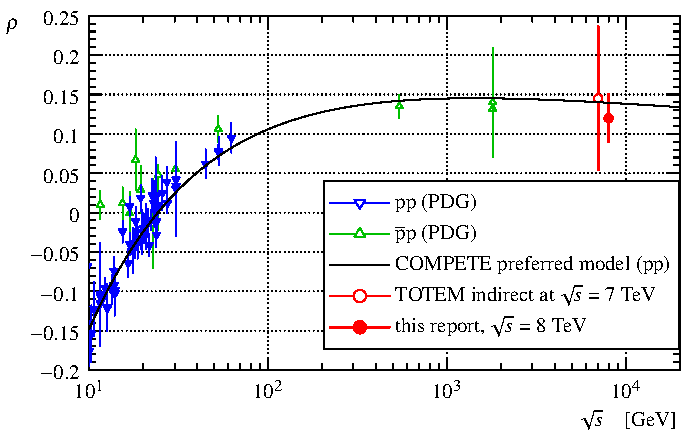
\includegraphics[width=16cm]{fig/rho_s.pdf}
\vspace*{3cm}
\vskip-3mm
\caption{$\rho$ as a function of $s$.}
\label{fig:rho_s}
\end{center}
\end{figure*}

\> figure for $\sigma_{\rm tot}$ result ??




%----------------------------------------------------------------------------------------------------

\subsubsection{Introduction}

In reference to the results published in the 90m run paper (or sections)... and in reference to the results published in the 1km paper (or sections)... we study in the present paper (or sections) a combined analysis of the Coulomb interference with the 90m and 1km data, with the objectives to:

\> investigate different combinations of: the formalization of the interference (SWY vs
KL), the models of the hadronic phase (central vs peripheral), and the functional
forms of the hadronic modulus (constant vs non-constant exponential at low-t);

\> extract physics quantities such as rho, total cross-section, and hadronic B slope, as
function of different assumptions on interference modelling and phase modelling;

\> quantify the various results in terms of C.L.

%----------------------------------------------------------------------------------------------------

\subsubsection{Elastic differential cross-section: 90m data + interference with Coulomb QED}

\todo{One needs to assume a rho value -- now we take 0.14, but later we will need to redo it with the result from 1km.}

We observe in the data a non-constant-exponential \& oscillating behaviour.
The hadronic slope by itself, the interference by itself, or a combination of both, must be
responsible for this effect.

\iffalse
{\bf 1. Fit with KL or SWY interference, constant/central phase, constant B slope}

Figures \ref{fig:90,SWY,con,1} and \ref{fig:90,KL,con,1}: statistical+systematic –based fitting exclude with high significance that the data can be
consistent with a constant B slope and constant phase. This is the case no matter which
interference formula is used. (rho is fixed to the Compete value).

\begin{figure*}
\begin{center}
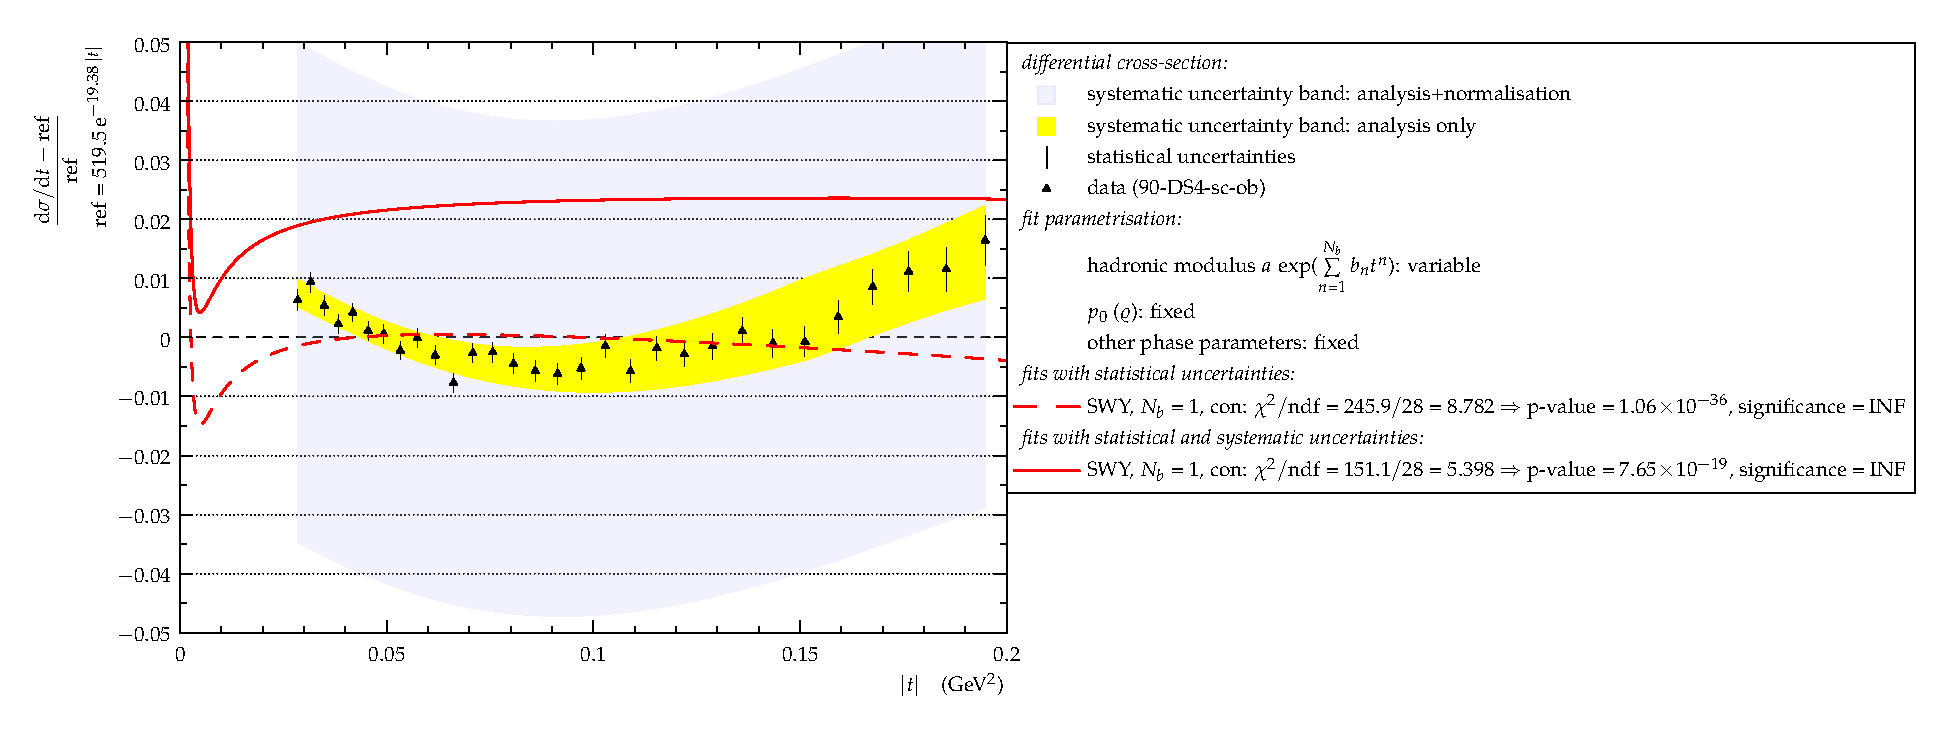
\includegraphics[width=18cm]{simone/90/SWY,con,1,stat-stat+syst.pdf}
\vskip-3mm
\caption{SWY formula, constant phase, 1 parameter in exponential}
\label{fig:90,SWY,con,1}
\end{center}
\end{figure*}

\begin{figure*}
\begin{center}
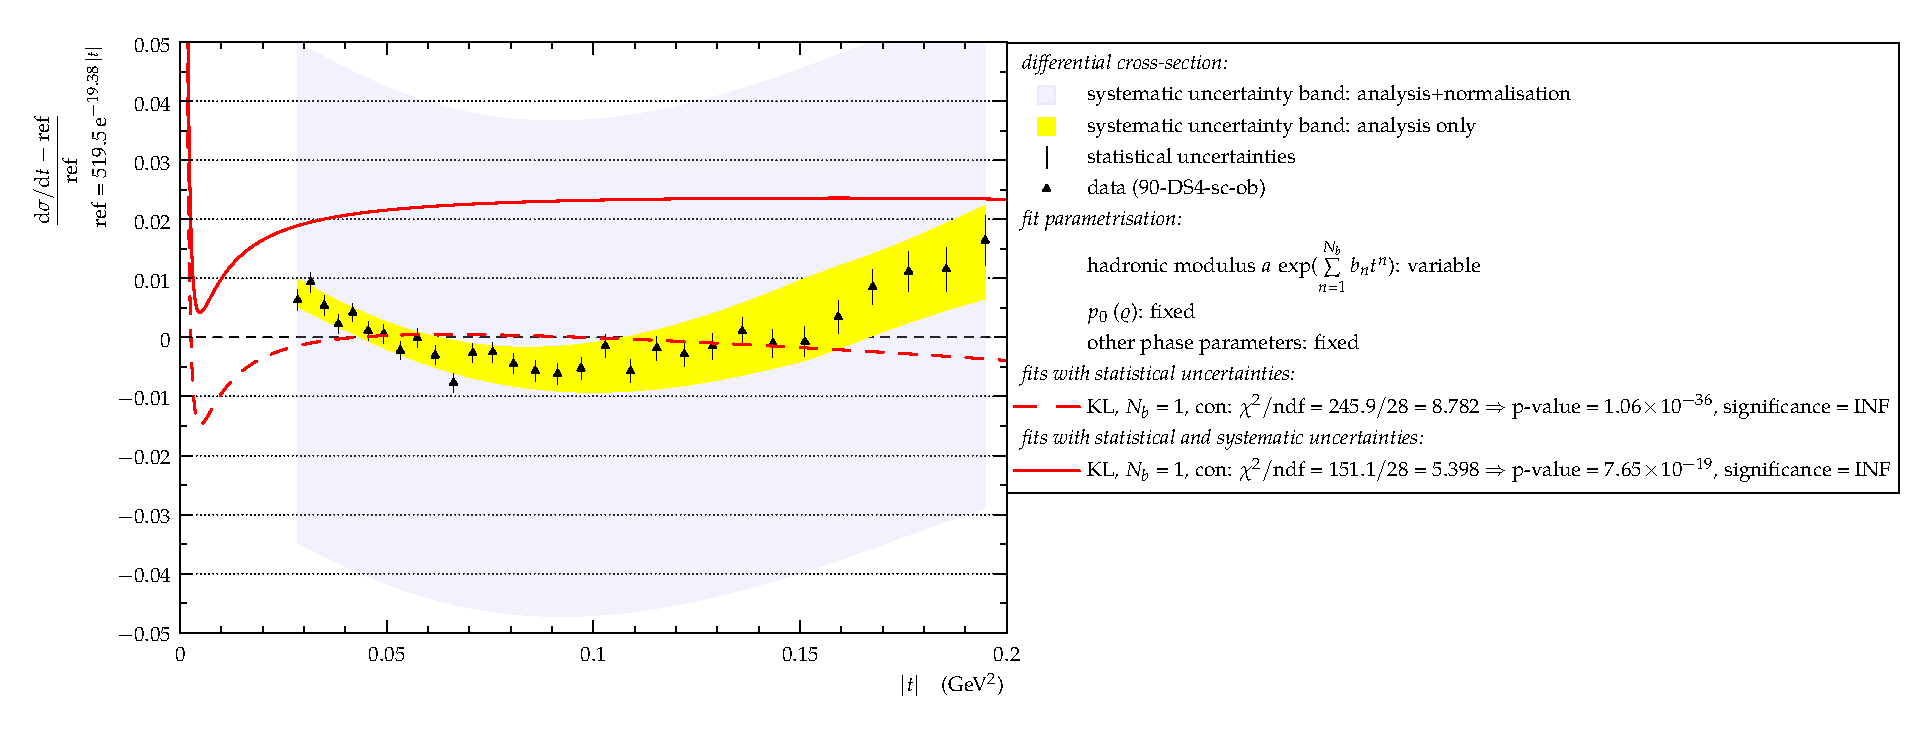
\includegraphics[width=18cm]{simone/90/KL,con,1,stat-stat+syst.pdf}
\vskip-3mm
\caption{KL formula, constant phase, 1 parameter in exponential}
\label{fig:90,KL,con,1}
\end{center}
\end{figure*}

SWY can only cope with constant B slope and constant phase, therefore it will not be
considered in the following.

Thus we will now consider only the KL interference formula, with central or peripheral
phase, with constant and not constant B slope.

For the peripheral phase, a range of 3 parameters qualified by physics properties in the impact
parameter space will be used. Later we will try a best fit with the 3 parameters constrained in
the given physical range.

For the B slope, 1 parameter (i.e. const) and 2-3-parameters functional forms will be used.

{\bf 2. Fit with KL interference, constant/central phase, non-constant B slope}

Figure \ref{fig:90,KL,con,2-3}: statistical only, and statistical+systematic, fitting for slope with 2 and 3 parameters. (rho is
fixed to the Compete value). Show/compare chi2, significance, C.L.

\begin{figure*}
\begin{center}
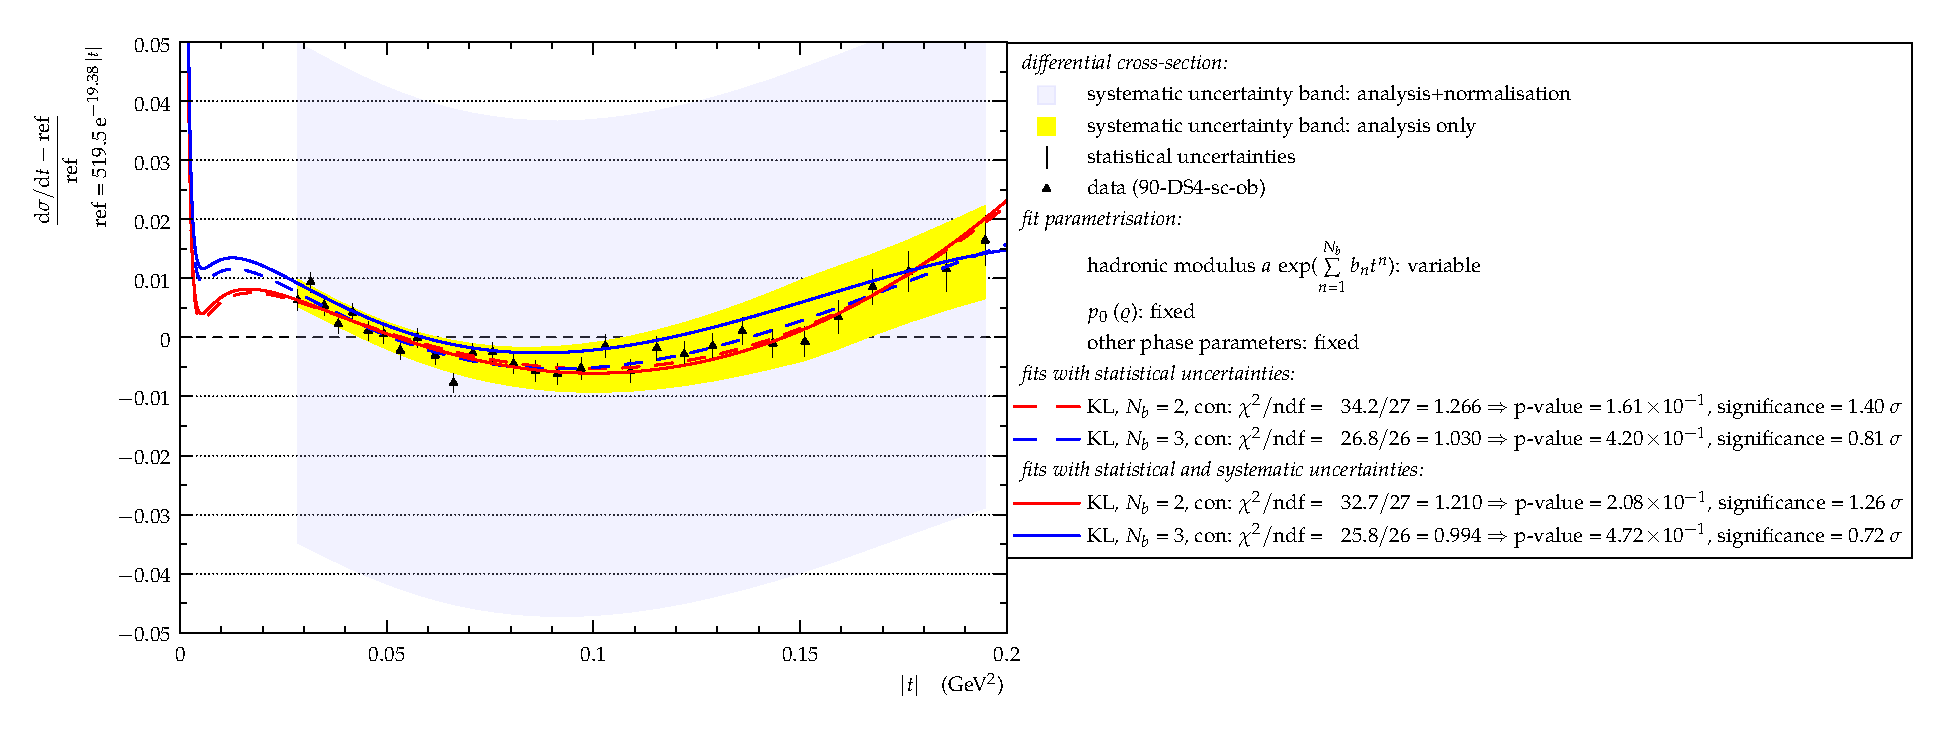
\includegraphics[width=18cm]{simone/90/KL,con,2-3,stat-stat+syst.pdf}
\vskip-3mm
\caption{KL formula, constant phase, 2 to 3 parameters in exponential}
\label{fig:90,KL,con,2-3}
\end{center}
\end{figure*}

{\bf 3. Fit with KL interference, peripheral phase, constant B slope}

Figure \ref{fig:90,KL,per,1}
statistical only and statistical+systematic fitting for constant slope, having fixed rho to the
Compete value and the other three phase parameters to the triplet in VK’s table first
row, or to the triplet in the central row, or to the triplet in the bottom row (to explore the
range and phase-space presented by VK at Collaboration Meetings).
Show/compare chi2, significance, C.L., ...

\begin{figure*}
\begin{center}
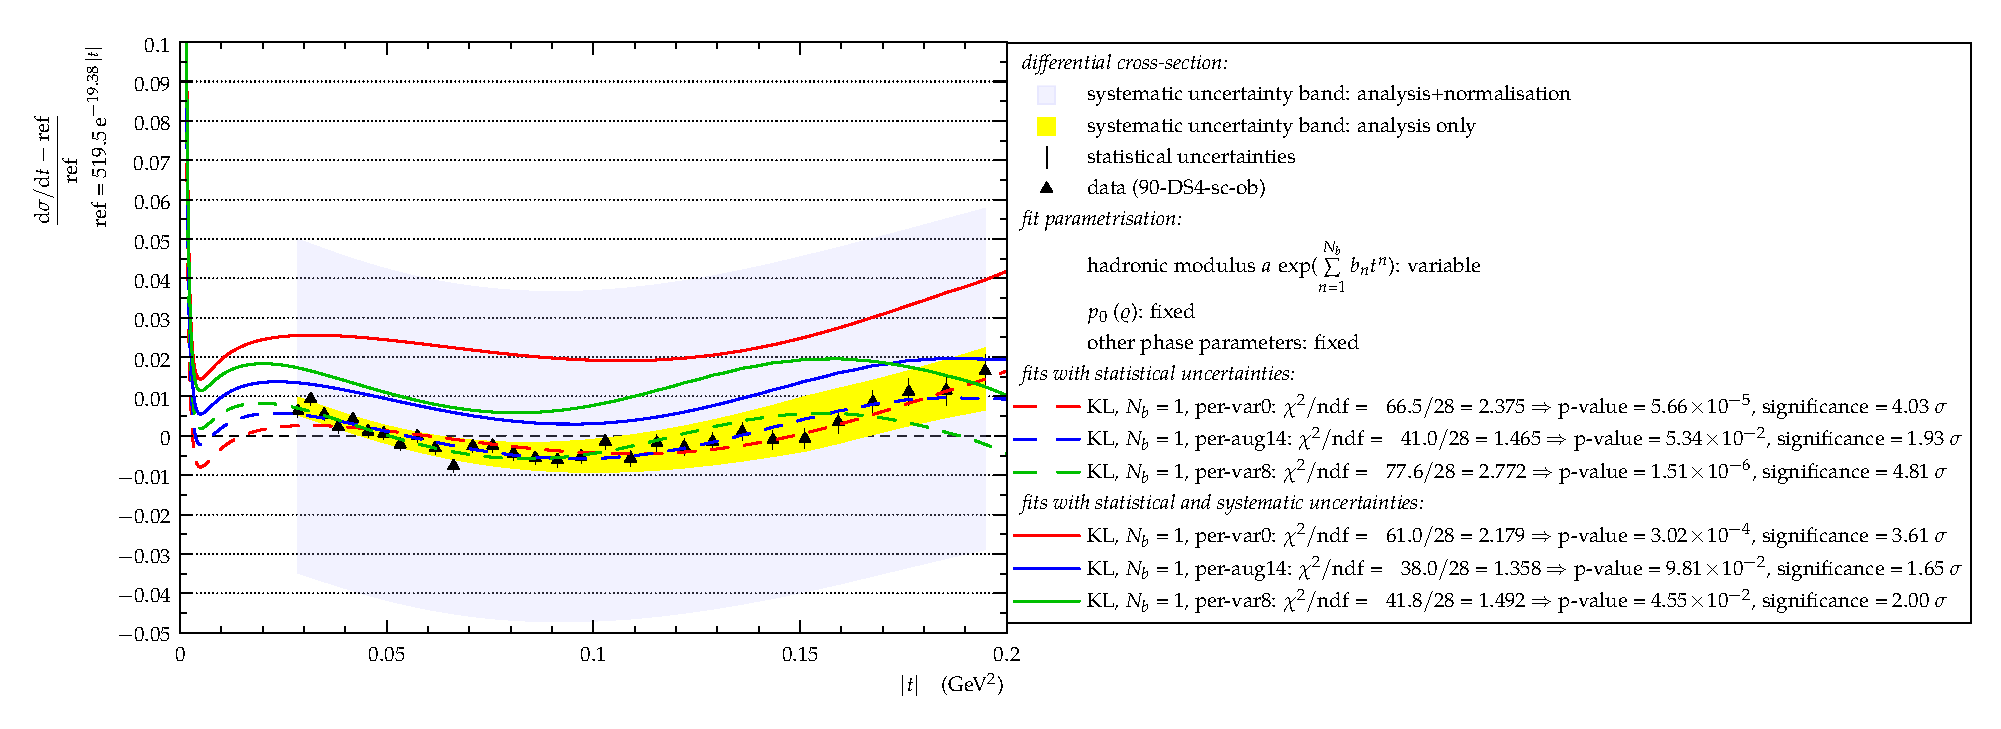
\includegraphics[width=18cm]{simone/90/KL,per-var048,1,stat-stat+syst.pdf}
\vskip-3mm
\caption{SWY formula, peripheral phases, 1 parameter in exponential}
\label{fig:90,KL,per,1}
\end{center}
\end{figure*}

{\bf 4. Fit with KL interference, peripheral phase, non-constant B slope}

\begin{figure*}
\begin{center}
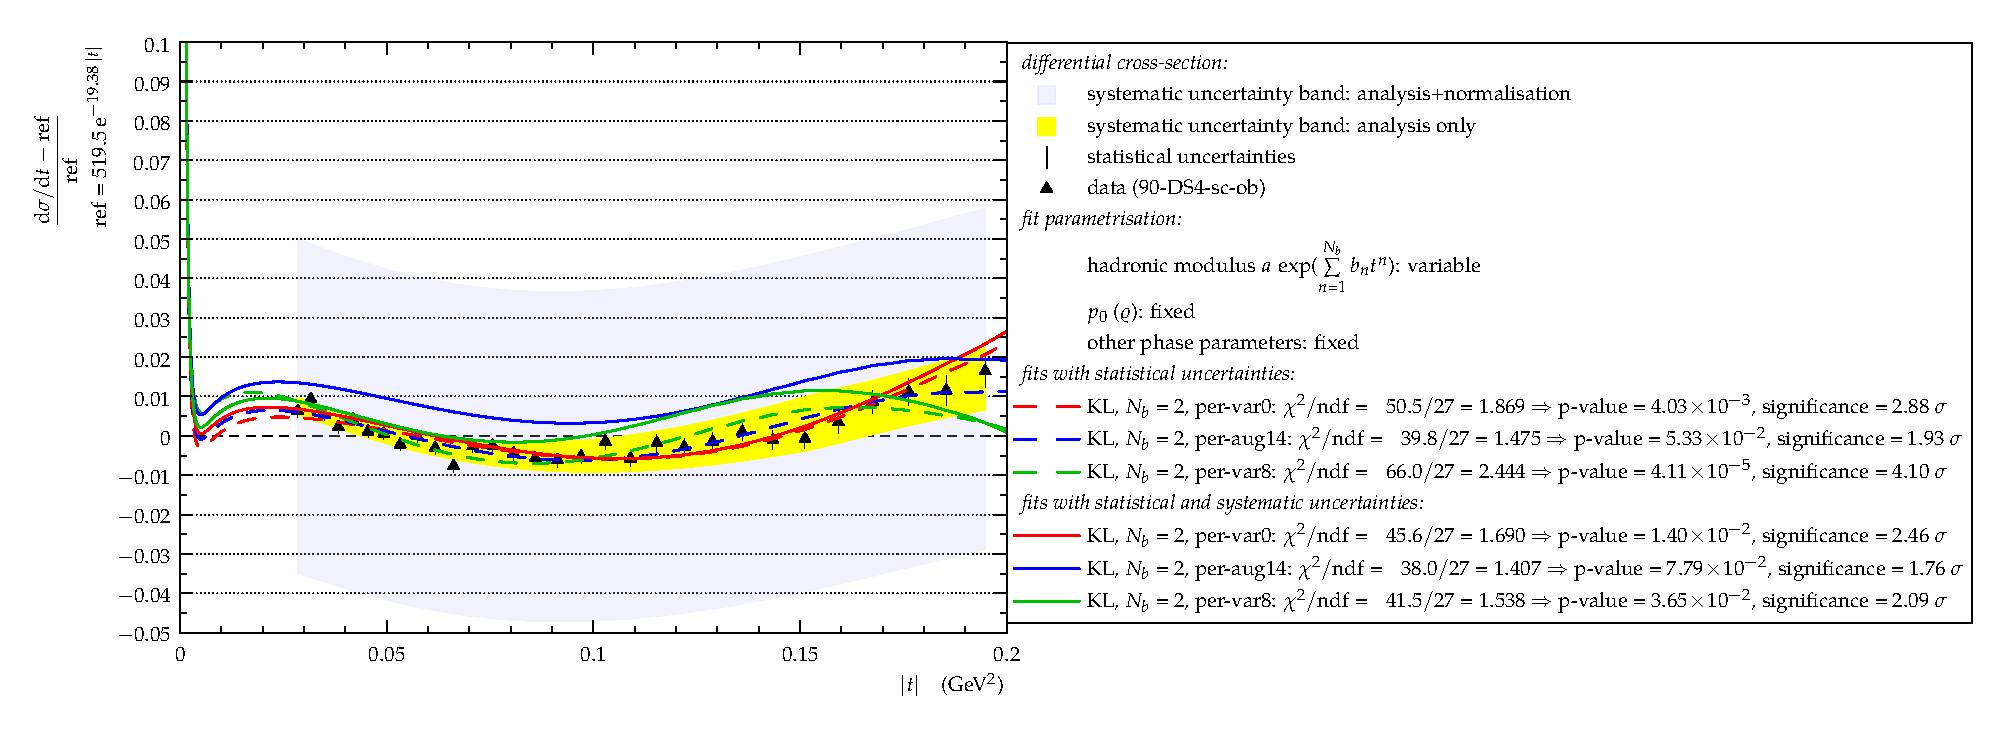
\includegraphics[width=18cm]{simone/90/KL,per-var048,2,stat-stat+syst.pdf}
\vskip-3mm
\caption{SWY formula, peripheral phases, 2 parameters in exponential}
\label{fig:90,KL,per,2}
\end{center}
\end{figure*}

\begin{figure*}
\begin{center}
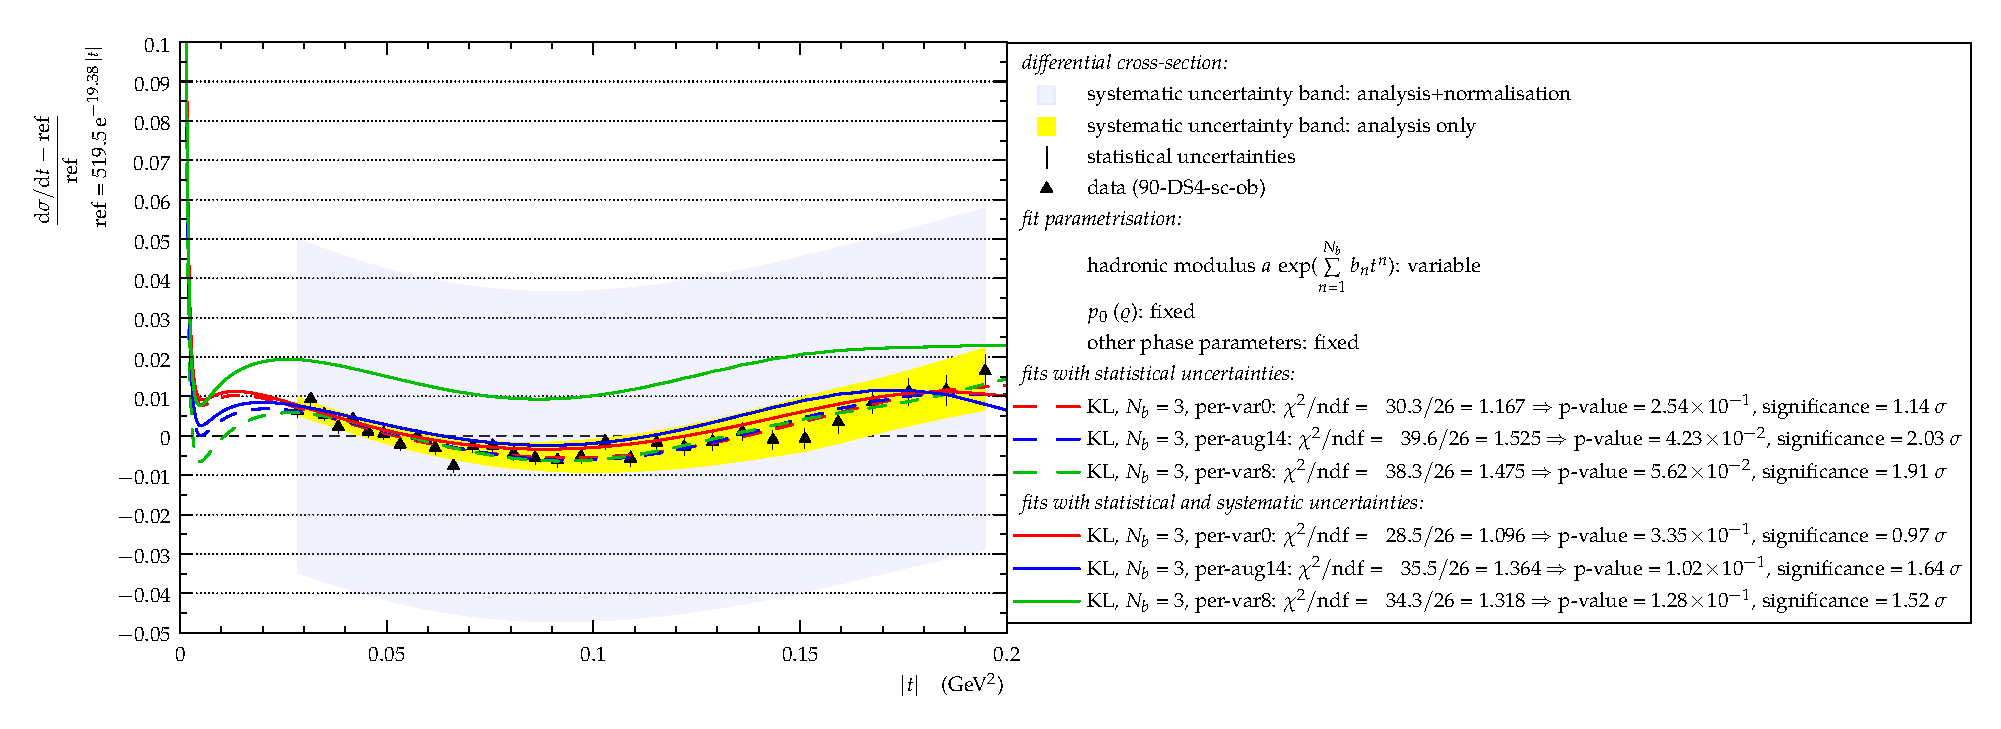
\includegraphics[width=18cm]{simone/90/KL,per-var048,3,stat-stat+syst.pdf}
\vskip-3mm
\caption{SWY formula, peripheral phases, 3 parameters in exponential}
\label{fig:90,KL,per,3}
\end{center}
\end{figure*}
\fi

Figures \ref{fig:90,KL,per,2} and \ref{fig:90,KL,per,3}:
statistical only and statistical+systematic fitting for slope with 2 and 3 parameters,
having fixed rho to the Compete value and the other three phase parameters to the triplet
in VK’s table first row, or to the triplet in the central row, or to the triplet in the
bottom row. Show/compare chi2, significance, C.L.,...

Check results by fixing rho to a different value, e.g. to the one resulting from the 1km
standalone data (under the traditional assumptions for the interference).

Concluding remarks on coupling of conditions and their significance.

%----------------------------------------------------------------------------------------------------

\subsubsection{Elastic differential cross-section: 90m \& 1km data + interference with Coulomb QED}

Repeat as above. Reciprocally constraining fits giving weight to the 90km or to the 1km data
for different physics quantities. Ultimately try combined fit properly weighting different
“experiments”.

%----------------------------------------------------------------------------------------------------

\subsubsection{Measurements of Rho, B, and Total Cross-Section}

Conditional analysis and results for the combinations analysed in the previous sections,
according to the sets of fits 1., 2., 3., 4.
